\documentclass[../main.tex]{subfiles}

\begin{document}

\section{Component Design}

\subsection{Meeple}

\begin{figure}[!htb]
    \centering
    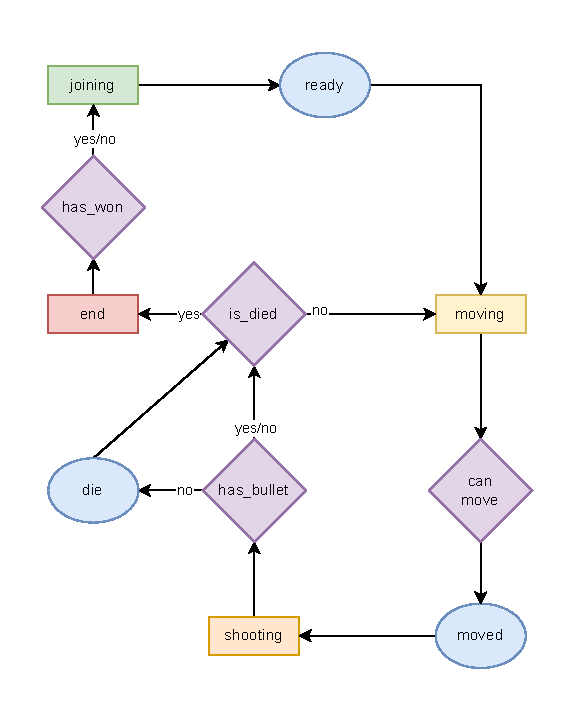
\includegraphics[width= 0.8\linewidth]{\subfix{../media/figures/meeple-logic.pdf}}\
    \caption{Meeple logic flow diagram}
    \label{fig:meeple-logic}
\end{figure}

The meeple is the component that represents the player position on the board and gives feedback about player movement, death and turn role; to do so, it uses two LEDs, a green one and a yellow one, and a hall sensor. To communicate with the game controller, it uses the MQTT protocol.

The meeple had a dedication time of around 10 hours, and was developed solely by Christian. It was a simple component to develop, but because of my lack of experience with electronics and cpp, it took me a while to get it working while trying to make the code scalable (and understandable). As stated before, the most challenging part was the making the CPP code work as intended, but also the ``blinking'' effect of the green LED.

\subsection{Operation base}

\begin{figure}[!htb]
    \centering
    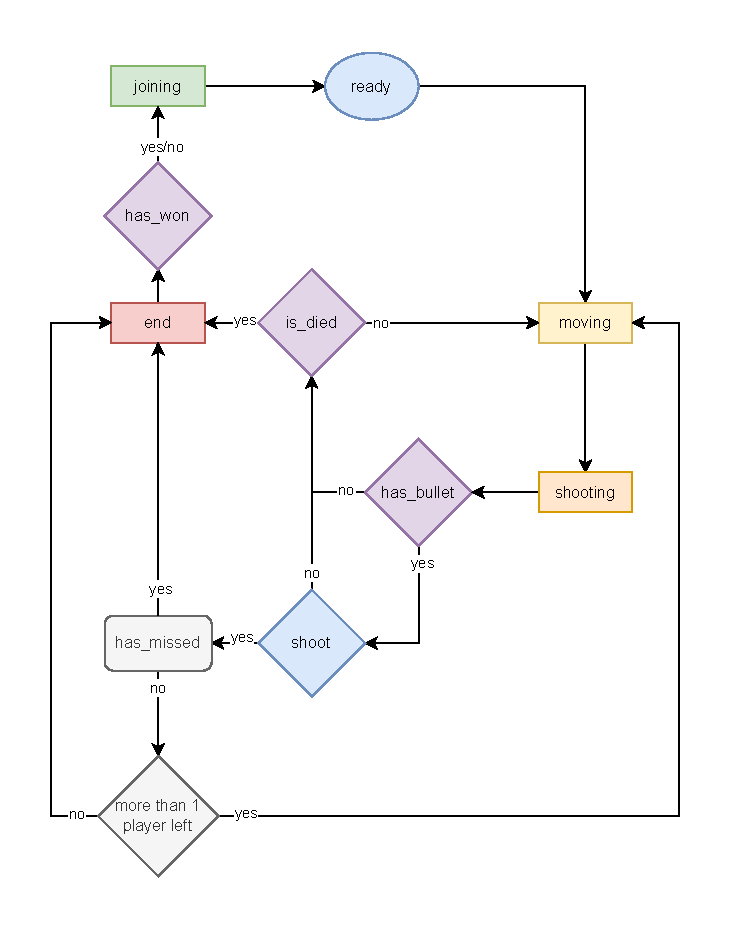
\includegraphics[width= 0.8\linewidth]{\subfix{../media/figures/base-logic.pdf}}\
    \caption{Operation base logic flow diagram}
    \label{fig:base-logic}
\end{figure}

\subsection{Game Controller}

\begin{figure}[!htb]
    \centering
    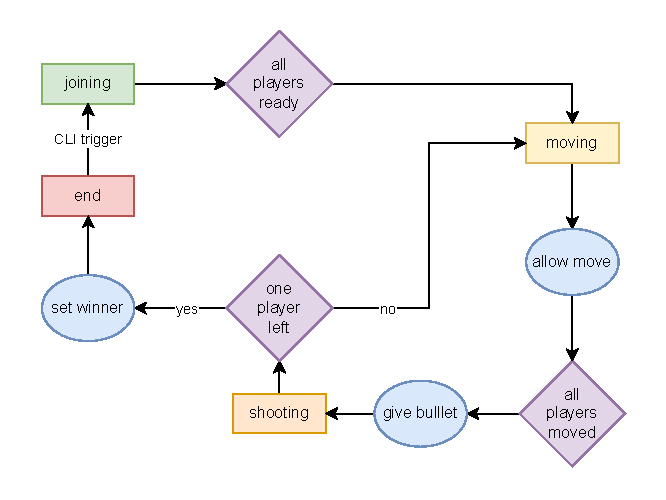
\includegraphics[width= 0.8\linewidth]{\subfix{../media/figures/master-logic.pdf}}\
    \caption{Master logic flow diagram}
    \label{fig:master-logic}
\end{figure}

This is the main component of the game, it controls the game flow, the player turns, the game state and communicates with the player feedback. It's a Docker container that runs a Python script using the MQTT protocol in a reactive way to communicate bidirectionally with the players. 

The game controller had a dedication of around 20 hours, and was developed solely by Christian. In the sense of the programming language, we chose Python because it didn't have to be inside any microchip so the speed didn't matter much, and because I am more experienced with it, even though I had never used the paho-mqtt library. The most challenging part was making a decent structure for the project, because I had some trouble with the circular imports trying to make the code understandable enough (I think I failed in this aspect in some parts). As I developed the meeple and the game controller parallely, I could test the communication between those two and I think that was good, but I could not test the game controller with any operation base, so I am not so sure about them working as expected. 

\subsection{Broker}

\end{document}